\section{Треугольники}

\subsection*{Понятие о многоугольнике и треугольнике}

\paragraph{Ломаная линия.}\label{1938/33}
Линия, образуемая отрезками, не лежащими на одной прямой и расположенными так, что конец первого служит началом второго, конец второго — началом третьего и~т.~д., называется \rindex{ломаная}\textbf{ломаной линией} (рис.~\ref{1938/ris-31} и \ref{1938/ris-32}).
Эти отрезки называются \rindex{сторона!ломаной}\textbf{сторонами} ломаной или её \rindex{звено}\textbf{звеньями}, а вершины углов, образуемых соседними отрезками, — \rindex{вершина!ломаной}\textbf{вершинами} её.
Ломаная линия обозначается рядом букв, поставленных у её вершин и концов;
например говорят:
ломаная $ABCDE$.
Ломаная линия называется \rindex{выпуклая ломаная}\textbf{выпуклой}, если она вся расположена по одну сторону от каждого входящего в её состав отрезка, продолженного неограниченно в обе стороны.
Такова, например, линия, изображённая на рис.~\ref{1938/ris-31}, тогда как ломаная на рис.~\ref{1938/ris-32} не будет выпуклой (она расположена не по одну сторону от прямой $BC$), рис.~\ref{1938/ris-31}.

\begin{figure}[h]
\begin{minipage}{.48\textwidth}
\centering
\includegraphics{mppics/ris-31}
\end{minipage}\hfill
\begin{minipage}{.48\textwidth}
\centering
\includegraphics{mppics/ris-32}
\end{minipage}

\medskip

\begin{minipage}{.48\textwidth}
\centering
\caption{}\label{1938/ris-31}
\end{minipage}\hfill
\begin{minipage}{.48\textwidth}
\centering
\caption{}\label{1938/ris-32}
\end{minipage}
\vskip-4mm
\end{figure}

Когда концы ломаной сходятся в одну точку, то она называется \rindex{замкнутая ломаная}\textbf{замкнутой} (например, линия $ABCDE$ на рис.~\ref{1938/ris-33}).

\paragraph{Многоугольник.}\label{1938/34}\rindex{многоугольник}
Фигура, образованная замкнутой ломаной линией вместе с частью плоскости, ограниченной этой линией, называется многоугольником (рис.~\ref{1938/ris-33}).
Стороны этой ломаной называются \rindex{сторона!многоугольника}\textbf{сторонами} многоугольника, углы, составленные каждыми двумя соседними сторонами, — \rindex{угол!многоугольника}\textbf{углами} многоугольника, а их вершины — \rindex{вершина!многоугольника}\textbf{вершинами} его.

\begin{figure}[!ht]
\centering
\includegraphics{mppics/ris-33}
\caption{}\label{1938/ris-33}
\end{figure}

При этом внутренней областью угла многоугольника считается (рис. \ref{1938/ris-33}) та, к которой принадлежит непосредственно примыкающая к вершине внутренняя область самого многоугольника.
Так, для многоугольника $MNPQRS$ (рис.~\ref{1938/ris-33}) углом при вершине $P$ является угол, больший двух прямых (с заштрихованной внутренней областью).
Сама ломаная линия, ограничивающая многоугольник, называется \rindex{контур многоугольника}\textbf{контуром} его, а отрезок, равный сумме всех его сторон, — \rindex{периметр}\textbf{периметром}.

Многоугольник называется \rindex{выпуклый многоугольник}\textbf{выпуклым}, если он ограничен выпуклой ломаной линией;
таков, например, многоугольник $ABCDE$, изображённый на рис.~\ref{1938/ris-33} (многоугольник $MNPQRS$ нельзя назвать выпуклым);
мы будем рассматривать, главным образом, выпуклые многоугольники.

Всякая прямая (как $AD$, $BE$, $MR,\dots$, рис.~\ref{1938/ris-33}), которая соединяет вершины двух углов многоугольника, не прилежащих к одной стороне, называется \rindex{диагональ}\textbf{диагональю} многоугольника.

Наименьшее число сторон в многоугольнике — три.
По числу сторон многоугольник называется \textbf{треугольником}, \textbf{четырёхугольником}, \textbf{пятиугольником} и~т.~д. Многоугольник с $n$ сторонами называется \rindex{$n$-угольник}\textbf{$\bm{n}$-угольником}. 

Для краткости «треугольник» обозначается символом $\triangle$;
например вместо «треугольник $ABC$» пишут «$\triangle ABC$».

\begin{figure}[!ht]
\begin{minipage}{.32\textwidth}
\centering
\includegraphics{mppics/ris-34}
\end{minipage}\hfill
\begin{minipage}{.32\textwidth}
\centering
\includegraphics{mppics/ris-35}
\end{minipage}\hfill
\begin{minipage}{.32\textwidth}
\centering
\includegraphics{mppics/ris-36}
\end{minipage}

\medskip

\begin{minipage}{.32\textwidth}
\centering
\caption{}\label{1938/ris-34}
\end{minipage}\hfill
\begin{minipage}{.32\textwidth}
\centering
\caption{}\label{1938/ris-35}
\end{minipage}\hfill
\begin{minipage}{.32\textwidth}
\centering
\caption{}\label{1938/ris-36}
\end{minipage}
\vskip-4mm
\end{figure}

\begin{wrapfigure}[11]{r}{50mm}
\vskip-4mm

\begin{minipage}{24mm}
\centering
\includegraphics{mppics/ris-ru-37}
\end{minipage}
\hfill
\begin{minipage}{24mm}
\centering
\includegraphics{mppics/ris-38}
\end{minipage}

\medskip

\begin{minipage}{24mm}
\centering
\caption{}\label{1938/ris-37}
\end{minipage}
\hfill
\begin{minipage}{24mm}
\centering
\caption{}\label{1938/ris-38}
\end{minipage}
\end{wrapfigure}

%%%%overfull
\paragraph{Типы треугольников.}\label{1938/35}
Треугольники разделяются по сравнительной длине их сторон или по величине их углов.
Относительно длины сторон они бывают:
\rindex{разносторонний треугольник}\textbf{разносторонние} (рис.~\ref{1938/ris-34}), когда все стороны различной длины, и \rindex{равнобедренный треугольник}\textbf{равнобедренные} (рис. \ref{1938/ris-35}), когда две стороны одинаковы;
в частности, равнобедренный треугольник называется \rindex{равносторонний треугольник}\textbf{равносторонним} (рис.~\ref{1938/ris-36}), когда все три его стороны равны между собой.

Относительно величины углов треугольники бывают:
\rindex{остроугольный треугольник}\textbf{остроугольные} (рис.~\ref{1938/ris-34}), когда все углы острые, \rindex{прямоугольный треугольник}\textbf{прямоугольные} (рис. \ref{1938/ris-37}), когда в числе углов есть прямой, и \rindex{тупоугольный треугольник}\textbf{тупоугольные} (рис.~\ref{1938/ris-38}), когда в числе углов есть тупой.

В прямоугольном треугольнике стороны, образующие прямой угол, называются \rindex{катет}\textbf{катетами}, а сторона, лежащая против прямого угла, — \rindex{гипотенуза}\textbf{гипотенузой}.

\paragraph{Основные линии в треугольнике.}\label{1938/36}
Одну из сторон треугольника иногда называют \rindex{основание!треугольника}\textbf{основанием}, тогда вершину противоположного угла называют \rindex{вершина}\textbf{вершиной} треугольника, а перпендикуляр, опущенный из вершины на основание или на его продолжение, — \rindex{высота!треугольника}\textbf{высотой} его.

Так, если в $\triangle ABC$ (рис.~\ref{1938/ris-39}) за основание взята сторона $AC$, то $B$ будет вершина, $BD$ — высота треугольника.

%%%%overfull
В равнобедренном треугольнике основанием называют обыкновенно ту сторону, которая не принадлежит к равным;
тогда вершина равнобедренного треугольника будет вершиной того угла его, который образован равными сторонами.
Отрезок $BE$ (рис.~\ref{1938/ris-39}), соединяющий вершину какого-нибудь угла треугольника с серединой противоположной стороны, называется \rindex{медиана}\textbf{медианой}.
Отрезок $BF$ (рис.~\ref{1938/ris-39}а), делящий какой-нибудь угол треугольника пополам, называется его \rindex{биссектриса!треугольника}\textbf{биссектрисой} (биссектриса, вообще говоря, не совпадает ни с медианой, ни с высотой).

\begin{figure}[!ht]
\centering
\includegraphics{mppics/ris-ru-39}
\caption{}\label{1938/ris-39}
\end{figure}

Из вершины каждого угла треугольника можно опустить перпендикуляр на противоположную сторону или её продолжение;
следовательно, каждый треугольник имеет три высоты.
Вершину каждого угла треугольника можно соединить прямой с серединой противоположной стороны, следовательно, каждый треугольник имеет три медианы.
Точно так же ясно, что каждый треугольник имеет три биссектрисы.

\subsection*{Осевая симметрия}



\begin{wrapfigure}{R}{49mm}
\centering
\includegraphics{mppics/ris-40}
\caption{}\label{1938/ris-40}
\end{wrapfigure}

\paragraph{}\label{1938/37}
При изучении свойств треугольников, многоугольников и других геометрических фигур часто встречается случай особого расположения на плоскости двух равных фигур или двух равных отрезков, или двух точек по отношению к какой-либо прямой.
Если какие-нибудь две точки $A$ и $A'$ (рис.~\ref{1938/ris-40}) расположены по разные стороны от прямой $MN$ на одном и том же перпендикуляре к этой прямой и на одинаковом расстоянии от основания перпендикуляра ($Aa=A'a$), то такие точки называются \rindex{симметрия относительно прямой}\textbf{симметричными} относительно прямой $MN$.

Две фигуры (или две части одной и той же фигуры) называются симметричными относительно прямой $MN$, если каждой точке $A$, $B$, $C$, $D$, $E,\dots$
(рис.~\ref{1938/ris-40}) одной фигуры (или одной части фигуры) соответствуют симметричные точки $A'$, $B'$, $C'$, $D'$, $E',\dots$ другой фигуры (или другой части фигуры), и обратно.
Прямая $MN$ в таком случае называется \rindex{ось симметрии}\textbf{осью симметрии}. 
Здесь слово «ось» применяется потому, что если часть плоскости, лежащую по одну сторону от прямой $MN$ (например, левую часть), станем вращать вокруг $MN$, как около оси, до тех пор, пока эта часть плоскости не упадёт на ту часть, которая лежит по другую сторону от прямой $MN$ (на правую часть), то симметричные фигуры совместятся, так как точка $A$ совпадёт при этом с точкой $A'$, точка $B$ — с точкой $B'$ и~т.~д.

Обратно, если вращением вокруг некоторой прямой мы можем фигуру, лежащую по одну сторону от этой прямой, совместить с фигурой, лежащей по другую её сторону, то эти фигуры симметричны относительно оси вращения.
Из сказанного следует, что

\textbf{\emph{всякие две фигуры, симметричные относительно какой-либо оси, равны между собой.}}

Симметрия относительно оси называется \rindex{осевая симметрия}\textbf{осевой симметрией}. 

\begin{wrapfigure}{o}{36mm}
\centering
\includegraphics{mppics/ris-41}
\caption{}\label{1938/ris-41}
\end{wrapfigure}

{\small
\smallskip
\mbox{\so{Замечание}.}
Хотя симметричные фигуры вращением вокруг оси симметрии могут быть приведены в совмещение, однако они, вообще говоря, не тождественны в своём расположении на плоскости.
Это нужно понимать в следующем смысле:
\emph{чтобы совместить две симметричные фигуры, необходимо одну из них перевернуть другой стороной и, следовательно, на время вывести её из плоскости.}
Если же не выводить фигуры из плоскости, то, вообще говоря, никаким перемещением в этой плоскости нельзя привести её к совпадению с фигурой, ей симметричной относительно оси.

На рис.~\ref{1938/ris-41} изображены два узора, симметричные относительно прямой $AB$.
Вращая правый узор около прямой $AB$, его можно совместить с левым узором.

При этом правый узор будет перевёрнут другой стороной.
Но если не отрывать правого узора от плоскости, а перемещать его так, чтобы он скользил по плоскости, то никаким передвижением его не удастся совместить с левым узором.

Осевая симметрия часто встречается в обыденной жизни.
Узоры на декоративных тканях и на комнатных обоях, архитектурные украшения на зданиях в виде плоских рисунков и самые фасады зданий имеют обычно форму, симметричную относительно некоторой оси.
В природе также часто встречаются симметричные формы.
Так, листья деревьев и лепестки цветов имеют форму, симметричную относительно среднего стебля.
Таков изображённый на рис.~\ref{1938/ris-42} лист клёна.
Крылья бабочки и их расцветка имеют форму, симметричную относительно оси её туловища (рис.~\ref{1938/ris-43}).

}

\begin{figure}[!ht]
\begin{minipage}{.48\textwidth}
\centering
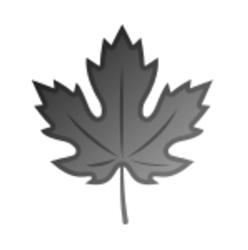
\includegraphics{eps/klenovyj-list}
\end{minipage}\hfill
\begin{minipage}{.48\textwidth}
\centering
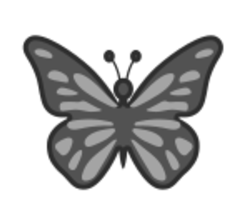
\includegraphics{eps/babochka}
\end{minipage}

\medskip

\begin{minipage}{.48\textwidth}
\centering
\caption{}\label{1938/ris-42}
\end{minipage}\hfill
\begin{minipage}{.48\textwidth}
\centering
\caption{}\label{1938/ris-43}
\end{minipage}
\vskip-4mm
\end{figure}

\subsection*{Свойства равнобедренного треугольника}

\paragraph{}\label{1938/38}
\so{Теоремы}.
1) \textbf{\emph{В равнобедренном треугольнике биссектриса угла при вершине есть одновременно и медиана и высота.}}

2) \textbf{\emph{В равнобедренном треугольнике углы при основании равны.}}

\begin{wrapfigure}{O}{36mm}
\centering
\includegraphics{mppics/ris-44}
\caption{}\label{1938/ris-44}
\end{wrapfigure}


Пусть $\triangle ABC$ (рис.~\ref{1938/ris-44}) равнобедренный и прямая $BD$ делит пополам угол $B$ при вершине его.
Требуется доказать, что эта биссектриса $BD$ есть также и медиана и высота.

Вообразим, что $\triangle ABD$ повёрнут вокруг стороны $BD$, как около оси, так, чтобы он упал на $\triangle BDC$.
Тогда, вследствие равенства углов 1 и 2, сторона $AB$ пойдёт по $BC$, а вследствие равенства этих сторон точка $A$ совпадёт с $C$.
Поэтому $BA$ совместится с $BC$, угол 4 совместится с углом 3 и угол 5 — с углом 6;
значит,
\[DA = BC,\quad \angle 4 = \angle 3\quad \text{и}\quad \angle 5 = \angle 6.\]

Из того, что $DA=DC$, следует, что $BD$ есть медиана;
из того, что углы 3 и 4 равны, вытекает, что эти углы прямые и, следовательно, $BD$ есть высота треугольника, и, наконец, углы 5 и 6 при основании треугольника равны.

\paragraph{}\label{1938/39}
\mbox{\so{Следствие}.}
Мы видим, что в равнобедренном треугольнике $ABC$ (рис.~\ref{1938/ris-44}) одна и та же прямая $BD$ обладает четырьмя свойствами:
она есть биссектриса угла при вершине, медиана, проведённая к основанию, высота, опущенная на основание, и, наконец, перпендикуляр к основанию, восстановленный из его середины. 
Перпендикуляр к отрезку, восстановленный из его середины называется \rindex{срединный перпендикуляр}\textbf{срединным перпендикуляром} к этому отрезку.

Так как каждое из этих четырёх свойств вполне определяет положение прямой $BD$, то существование одного из них влечёт все остальные.
Например, \emph{высота, опущенная на основание равнобедренного треугольника, служит одновременно биссектрисой угла при вершине, медианой, проведённой к основанию, и срединным перпендикуляром к основанию.} 

\paragraph{Симметрия равнобедренного треугольника.}\label{1938/40}
Мы видели, что равнобедренный $\triangle ABC$ (рис.~\ref{1938/ris-44}) делится биссектрисой $BD$ на такие два треугольника (левый и правый), которые вращением вокруг биссектрисы могут быть совмещены один с другим.
Из этого можно заключить, что какую бы точку на одной половине равнобедренного треугольника мы ни взяли, всегда можно на другой его половине найти точку, симметричную с первой относительно оси $BD$.
Возьмём, например, на стороне $AB$ точку $M$ (рис.~\ref{1938/ris-44}).
Опустим из неё на $BD$ перпендикуляр $MK$ и продолжим его до пересечения со стороной $BC$.
Мы получим тогда на этой стороне точку $M'$, симметричную с точкой $M$ относительно оси $BD$.
Действительно, если, вращая $\triangle ABD$ вокруг $BD$, мы его совместим с $\triangle BCD$, то при этом $KM$ пойдёт по $KM'$ (по равенству прямых углов), а сторона $BA$ пойдёт по стороне $BC$ (по равенству углов при вершине $B$);
значит, точка $M$, которая лежит на $KM$ и на $BA$, совпадёт с точкой $M'$, которая лежит и на $KM'$, и на $BC$.
Отсюда видно, что $KM=KM'$.
Таким образом, точки $M$ и $M'$ лежат по разные стороны от биссектрисы $BD$, на одном к ней перпендикуляре и на равных расстояниях от основания этого перпендикуляра;
значит, эти точки симметричны относительно оси $BD$.
Таким образом, \emph{в равнобедренном треугольнике биссектриса угла при вершине есть его ось симметрии.}


\subsection*{Признаки равенства треугольников}

\paragraph{Предварительные понятия.}\label{1938/41}
Две геометрические фигуры, например два треугольника, как мы знаем, называются равными, если они при наложении могут быть совмещены.
В совмещающихся треугольниках, конечно, должны быть соответственно равны все элементы их, то есть стороны, углы, высоты, медианы и биссектрисы.
Однако для того, чтобы утверждать, что два треугольника равны, нет необходимости устанавливать равенства всех их элементов, достаточно убедиться в равенстве только некоторых из них.


\paragraph{Признаки равенства треугольников.}\label{1938/42}\ 

1) \textbf{\emph{Если две стороны и угол, заключённый
между ними, одного треугольника соответственно равны
двум сторонам и углу, заключённому между ними, другого треугольника, то такие треугольники равны.}}

2) \textbf{\emph{Если два угла и прилежащая к ним сторона одного треугольника соответственно равны двум углам и прилежащей к ним стороне другого треугольника, то такие треугольники равны.}}

%%%%overfull
3) \textbf{\emph{Если три стороны одного треугольника равны трём сторонам другого треугольника, то такие треугольники равны.}}

1) Пусть $ABC$ и $A_1B_1C_1$ — два треугольника (рис.~\ref{1938/ris-45}), у которых
$AC\z=A_1C_1$, $AB \z= A_1B_1$, $\angle A \z= \angle A_1$.
Требуется доказать, что эти треугольники равны.
\begin{figure}[h]
\begin{minipage}{.48\textwidth}
\centering
\includegraphics{mppics/ris-45}
\end{minipage}\hfill
\begin{minipage}{.48\textwidth}
\centering
\includegraphics{mppics/ris-46}
\end{minipage}

\medskip

\begin{minipage}{.48\textwidth}
\centering
\caption{}\label{1938/ris-45}
\end{minipage}\hfill
\begin{minipage}{.48\textwidth}
\centering
\caption{}\label{1938/ris-46}
\end{minipage}
\vskip-4mm
\end{figure}

Наложим%
\footnote{Для выполнения указанных в этом параграфе наложений иногда приходится накладываемый треугольник перевернуть другой стороной.} 
$\triangle ABC$ на $\triangle A_1B_1C_1$ так, чтобы точка $A$ совпала с $A_1$ и сторона $AC$ пошла по $A_1C_1$.
Тогда, вследствие равенства этих сторон, точка $C$ совместится с $C_1$, вследствие равенства углов $A$ и $A_1$ сторона $AB$ пойдёт по $A_1B_1$, а вследствие равенства этих сторон точка $B$ совпадёт с $B_1$, поэтому сторона $CB$ совместится с $C_1B_1$ (так как две точки можно соединить только одной прямой), и треугольники совпадут;
значит, они равны.


2) Пусть $ABC$ и $A_1B_1C_1$ (рис.~\ref{1938/ris-46}) — два треугольника, у которых $\angle C= \angle C_1$,
$\angle B=\angle B_1$,
и
$CB = C_1B_1$.
Требуется доказать, что эти треугольники равны.

Наложим $\triangle ABC$ на $\triangle A_1B_1C_1$ так, чтобы точка $C$ совпала с $C_1$ и сторона $CB$ пошла по $C_1B_1$.
Тогда, вследствие равенства этих сторон, точка $B$ совпадёт с $B_1$, а вследствие равенства углов $B$ и $B_1$, $C$ и $C_1$, сторона $BA$ пойдёт по $B_1A_1$ и сторона $CA$ — по $C_1A_1$.


Так как две прямые могут пересечься только в одной точке, то вершина $A$ должна совпасть с $A_1$.
Таким образом, треугольники совместятся;
значит, они равны.

\begin{wrapfigure}{o}{35mm}
\vskip-0mm
\centering
\includegraphics{mppics/ris-47}
\caption{}\label{1938/ris-47}
\end{wrapfigure}

3) Пусть $ABC$ и $A_1B_1C_1$ (рис.~\ref{1938/ris-47}) — два треугольника, у которых
$AB \z= A_1B_1$,
$BC \z= B_1C_1$,
и
$CA = C_1A_1$.
Требуется доказать, что эти треугольники равны.

Доказывать этот признак равенства наложением, как мы это делали для первых признаков, было бы неудобно, так как, не зная ничего о величине углов, мы не можем утверждать, что при совпадении двух равных сторон совпадут и остальные стороны.
Вместо наложения применим здесь \textbf{приложение}.

Приложим $\triangle ABC$ к $\triangle A_1B_1C_1$ так, чтобы у них совместились равные стороны $AC$ и $A_1C_1$.
Тогда $\triangle ABC$ займёт положение $\triangle A_1C_1B_2$.

Соединив прямой точки $B_1$ и $B_2$, мы получим два равнобедренных треугольника $A_1B_1B_2$ и $B_1C_1B_2$ с общим основанием $B_1B_2$.
Но в равнобедренном треугольнике углы при основании равны (§~\ref{1938/38});
следовательно, $\angle 1 = \angle 2$ и $\angle 3 \z= \angle 4$, а потому $\angle A_1B_1C_1 = \angle A_1B_2C_1 = \angle B$.
Но в таком случае данные треугольники должны быть равны, так как две стороны и угол, заключённый между ними, одного треугольника соответственно равны двум сторонам и углу, заключённому между ними, другого треугольника.

\begin{wrapfigure}{r}{63mm}
\vskip-0mm
\begin{minipage}{31mm}
\centering
\includegraphics{mppics/ris-1914-40}
\end{minipage}\hfill
\begin{minipage}{31mm}
\centering
\includegraphics{mppics/ris-1914-41}
\end{minipage}
\medskip
\begin{minipage}{31mm}
\centering
\caption{}\label{1914/ris-40}
\end{minipage}\hfill
\begin{minipage}{31mm}
\centering
\caption{}\label{1914/ris-41}
\end{minipage}
\end{wrapfigure}

\medskip

%%%%overfull
Может случиться, что прямая $B_1B_2$ не пересечётся со стороной $A_1C_1$,
а пойдёт вне треугольников (если сумма углов $C$ и $C_1$, большее $180\degree$),
или сольётся с линией $B_1C_1B_2$ (если $\angle C +\angle  C_1 \z= 180\degree$). Доказательство остаётся то же самое, с той разницей, что углы $B_1$ и $B_2$
будут равны друг другу, не как \so{суммы} равных углов, а как их разности, (рис.~\ref{1914/ris-40}), или как углы при основании равнобедренного треугольника (рис.~\ref{1914/ris-41}).

{\small
\smallskip
\mbox{\so{Замечание}.}
\emph{В равных треугольниках против равных сторон лежат равные углы, и обратно, против равных углов лежат равные стороны.}

Доказанные теоремы о равенстве треугольников и умение распознавать равные треугольники по указанным признакам чрезвычайно облегчают решение многих геометрических задач и необходимы для доказательства многих теорем.
Теоремы о равенстве треугольников являются главным средством для обнаружения свойств сложных геометрических фигур.
Учащиеся убедятся в этом при дальнейшем прохождении предмета.
}

\subsection*{Внешний угол треугольника}

\paragraph{}\label{1938/43}
\mbox{\so{Определение}.}
Угол, смежный с каким-нибудь углом треугольника (или многоугольника), называется \rindex{внешний угол}\textbf{внешним} углом этого треугольника (или многоугольника). 

Таковы, например, углы $BCD$, $CBE$, $BAF$ (рис.~\ref{1938/ris-48}).
В отличие от внешних углы самого треугольника (или многоугольника) называются \rindex{внутренний угол}\textbf{внутренними}. 

При каждом угле треугольника (или многоугольника) можно построить по два внешних угла (продолжив одну или другую сторону угла).
Эти два угла равны, как углы вертикальные.

\begin{figure}[!ht]
\begin{minipage}{.48\textwidth}
\centering
\includegraphics{mppics/ris-48}
\end{minipage}\hfill
\begin{minipage}{.48\textwidth}
\centering
\includegraphics{mppics/ris-49}
\end{minipage}

\begin{minipage}{.48\textwidth}
\centering
\caption{}\label{1938/ris-48}
\end{minipage}\hfill
\begin{minipage}{.48\textwidth}
\centering
\caption{}\label{1938/ris-49}
\end{minipage}
\end{figure}

\paragraph{}\label{1938/44}
\mbox{\so{Теорема}.}
\textbf{\emph{Внешний угол треугольника больше каждого внутреннего угла его, не смежного с этим внешним.}}


Например, докажем, что внешний угол $BCD$ треугольника $ABC$
(рис.~\ref{1938/ris-49}) больше каждого из внутренних углов $A$ и $B$, не смежных с этим внешним.

Через середину $E$ стороны $BC$ проведём медиану $AE$ и на её продолжении отложим отрезок $EF=AE$.
Точка $E$, очевидно, будет лежать внутри угла $BCD$.
Соединим $E$ с $C$ прямой.
Треугольники $ABE$ и $EFC$ (покрытые штрихами) равны, так как при точке $E$ они имеют по равному углу, заключённому между двумя соответственно равными сторонами.
Из равенства их заключаем, что углы $B$ и $ECF$, лежащие против равных сторон $AE$ и $EF$, равны.
Но угол $ECF$ составляет часть внешнего угла $BCD$ и потому меньше его;
следовательно, и угол $B$ меньше угла $BCD$.



Продолжив сторону $BC$ за точку $C$, мы получим внешний угол $ACH$, равный углу $BCD$.
Если из вершины $B$ проведём к стороне $AC$ медиану и продолжим её на такую же длину за сторону $AC$, то совершенно так же докажем, что угол $A$ меньше угла $ACH$, то есть меньше угла $BCD$.

{

\begin{wrapfigure}[8]{r}{57mm}
\vskip-0mm
\begin{minipage}{28mm}
\centering
\includegraphics{mppics/ris-50}
\end{minipage}\hfill
\begin{minipage}{28mm}
\centering
\includegraphics{mppics/ris-51}
\end{minipage}
\medskip
\begin{minipage}{28mm}
\centering
\caption{}\label{1914/ris-50}
\end{minipage}\hfill
\begin{minipage}{28mm}
\centering
\caption{}\label{1914/ris-51}
\end{minipage}

\end{wrapfigure}

\paragraph{}\label{1938/45}
\mbox{\so{Следствие}.}
\emph{Если в треугольнике один угол прямой или тупой, то два других угла острые.}
Действительно, допустим, что угол $C$ треугольника $ABC$ 
(рис.~\ref{1914/ris-50} и \ref{1914/ris-51}) будет прямой или тупой, тогда смежный с ним внешний угол $BCD$ должен быть прямой или острый;
следовательно, углы $A$ и $B$, которые, по доказанному, меньше этого внешнего угла, должны быть оба острые.

}

\subsection*{Стороны и углы треугольника}

\paragraph{}\label{1938/46}
\so{Теоремы}.
\textbf{\emph{Во всяком треугольнике}}

\textbf{\emph{1) против равных сторон лежат равные углы.}}

\textbf{\emph{2) против б\'{о}льшей стороны лежит больший угол.}}

\begin{wrapfigure}{o}{33mm}
\vskip-4mm
\centering
\includegraphics{mppics/ris-52}
\caption{}\label{1938/ris-52}
\bigskip
\includegraphics{mppics/ris-53}
\caption{}\label{1938/ris-53}
\end{wrapfigure}

1) Если две стороны треугольника равны, то он равнобедренный, тогда углы, лежащие против этих сторон, должны быть равны, как углы при основании равнобедренного треугольника (§~\ref{1938/38}).

2) Пусть в $\triangle ABC$ (рис.~\ref{1938/ris-52}) сторона $AB$ больше $BC$;
требуется доказать, что угол $C$ больше угла $A$.

Отложим на б\'{о}льшей стороне $BA$ от вершины $B$ отрезок $BD$, равный меньшей стороне $BC$, и соединим $D$ с $C$ прямой.
Тогда получим равнобедренный $\triangle BDC$, у которого углы при основании равны, то есть $\angle BDC=\angle BCD$.
Но угол $BDC$ как внешний по отношению к $\angle ADC$, больше угла $A$, следовательно, и угол $BCD$ больше угла $A$, а потому и подавно угол $BCA$ больше угла $A$, что и требовалось доказать.

\paragraph{}\label{1938/47}
\mbox{\so{Обратные теоремы}.}
\textbf{\emph{Во всяком треугольнике.}}

1) \textbf{\emph{против равных углов лежат равные стороны;}}

2) \textbf{\emph{против б\'{о}льшего угла лежит б\'{о}льшая сторона.}}

1) Пусть в $\triangle ABC$ углы $A$ и $C$ равны (рис.~\ref{1938/ris-53});
требуется доказать, что $BA \z= BC$.

Предположим противное, то есть что стороны $AB$ и $BC$ не равны.
Тогда одна из этих сторон должна быть больше другой, и, следовательно, согласно прямой теореме, один из углов $A$ и $C$ должен быть больше другого.
Но это противоречит условию, что $\angle A = \angle C$;
значит, нельзя допустить, что стороны $AB$ и $BC$ не равны;
остаётся принять, что $AB=BC$.


2) Пусть в $\triangle ABC$ (рис.~\ref{1938/ris-54})
угол $C$ больше угла $A$;
требуется доказать, что $AB > BC$.

{

\begin{wrapfigure}[10]{r}{30mm}
\centering
\includegraphics{mppics/ris-54}
\caption{}\label{1938/ris-54}
\end{wrapfigure}

Предположим противное, то есть что $AB$ не больше $BC$.
Тогда могут представиться два случая:
или $AB=BC$, или $AB<BC$.

В первом случае, согласно прямой теореме, угол $C$ был бы равен углу $A$, во втором случае угол $C$ был бы меньше угла $A$;
и то и другое противоречит условию;
значит, оба эти случая исключаются.
Остаётся один возможный случай, что $AB>BC$.

\smallskip
\mbox{\so{Следствия}.}
1) \emph{В равностороннем треугольнике все углы равны.}

2) \emph{В равноугольном треугольнике все стороны равны.}

}

{\sloppy
\paragraph{Доказательство от противного.}\label{1938/48}
Способ, которым мы только что доказали обратные теоремы, называется \rindex{доказательство от противного}\textbf{доказательством от противного}, или приведением к \rindex{противоречие}\textbf{противоречию}.
Первое название этот способ получил потому, что в начале рассуждения делается предположение, противное (противоположное) тому, что требуется доказать.
Приведением к противоречию он называется вследствие того, что, рассуждая на основании сделанного предположения, мы приходим к противоречию (к абсурду).
Получение такого вывода заставляет нас отвергнуть сделанное вначале допущение и принять то, которое требовалось доказать.

}

Этот приём очень часто употребляется для доказательства теорем.

\paragraph{Замечание об обратных теоремах.}\label{1938/49}
Начинающие изучать геометрию часто делают одну характерную ошибку.
Она заключается в том, что правильность обратной теоремы считают само собой разумеющейся, если доказана прямая теорема.
Отсюда представление, что доказательство обратных теорем вообще излишне.
Ошибочность такого заключения может быть показана в ряде примеров.
В частности, такой пример был приведён в §~\ref{1938/30}.
Поэтому обратные теоремы, когда они верны, всегда доказываются особо.



\subsection*{Длина ломаной}

\paragraph{}\label{1938/50}
\so{Теорема}.
\textbf{\emph{В треугольнике каждая сторона меньше суммы двух других сторон.}}

Если в треугольнике возьмём сторону не самую большую, то, конечно, она окажется менее суммы двух других сторон.
Значит, нам надо доказать, что даже \so{наибольшая} сторона треугольника меньше суммы двух других сторон.

Пусть в $\triangle ABC$ (рис.~\ref{1938/ris-55}) наибольшая сторона есть $AC$.
Продолжив сторону $AB$, отложим $BD=BC$ и проведём $DC$.
Так как $\triangle BDC$ равнобедренный, то $\angle D = \angle DCB$;
поэтому угол $D$ меньше угла $DCA$, и, следовательно, в $\triangle ADC$ сторона $AC$ меньше $AD$ (§~\ref{1938/47}), то есть
$AC \z< AB + BD$.
Заменив $BD$ на $BC$, получим:
\[AC < AB + BC.\]

\begin{wrapfigure}{o}{33mm}
\vskip-8mm
\centering
\includegraphics{mppics/ris-55}
\caption{}\label{1938/ris-55}
\end{wrapfigure}

\smallskip
\mbox{\so{Следствие}.}
Отнимем от обеих частей выведенного неравенства по $AB$ или по $BC$:
\begin{align*}
AC-AB&<BC;
\\
AC-BC&<AB.
\end{align*}
Читая эти неравенства справа налево, видим, что каждая из сторон $BC$ и $AB$ больше разности двух других сторон;
так как это же можно, очевидно, сказать и о третьей, наибольшей стороне $AC$, то, значит, \emph{в треугольнике каждая сторона больше разности двух других сторон.}


\paragraph{Неравенство треугольника}\label{extra/3inq}
\emph{Для любых трёх точек $A$, $B$ и $C$ выполняется неравенство
\[AC \le AB + BC;\]
то есть отрезок $AC$ может быть равен сумме $AB + BC$ или больше неё.
При этом равенство достигается только в случае если $B$ лежит на отрезке $AC$.}
Это неравенство называется \rindex{неравенство треугольника}\textbf{неравенством треугольника}.

Случай когда $B$ не лежит на прямой $AC$ (то есть если $A$, $B$ и $C$ являются вершинами некоторого треугольника) уже доказан (§~\ref{1938/50}). 
Остаётся рассмотреть случай когда $B$ лежит на прямой $AC$.

Равенство 
\[AC = AB + BC;\]
очевидно выполняется в случае если $B$ лежит на отрезке $AC$.
В случае если $B$ лежит на продолжении отрезка $AC$, то очевидно
$AC=AB\z-BC<AB$ или $AC=CB-BA<CB$;
в обоих случаях имеем
\[AC < AB + BC.\] 

\paragraph{}\label{1938/51}
\mbox{\so{Теорема}.}
\textbf{\emph{Отрезок, соединяющий две какие-нибудь точки, меньше всякой ломаной, соединяющей эти же точки.}}

Если ломаная состоит только из двух сторон, то теорема уже была доказана в предыдущем параграфе.
Рассмотрим случай, когда ломаная состоит более чем из двух сторон.
Пусть $AE$ (рис.~\ref{1938/ris-56}) есть отрезок, соединяющий точки $A$ и $E$, а $ABCDE$ — какая-нибудь ломаная, соединяющая те же точки.
Требуется доказать, что 
\[AE<AB\z+BC\z+CD\z+DE.\eqno(1)\]

{

\begin{wrapfigure}{r}{33mm}
\vskip0mm
\centering
\includegraphics{mppics/ris-56}
\caption{}\label{1938/ris-56}
\end{wrapfigure}

Соединив $A$ с $C$ и $D$, находим, согласно неравенству треугольника (§~\ref{extra/3inq})
\begin{align*}
AE&\le AD+DE;
\\
AD&\le AC +CD;
\\
AC&< AB+BC.
\end{align*}
Последнее неравенство строгое поскольку $B$ не может лежать на отрезке $AC$.

}

Сложим почленно эти неравенства и затем от обеих частей полученного неравенства отнимем по $AD$ и $AC$; тогда получим неравенство~(1).


\paragraph{Треугольники с двумя соответственно равными сторонами.}\label{1938/52}\ 

\smallskip
\so{Теоремы}.
\textbf{\emph{Если две стороны одного треугольника соответственно равны двум сторонам другого треугольника, то:}}

1) \textbf{\emph{против большего из углов, заключённых между ними, лежит б\'{о}льшая сторона.}}

2) \so{обратно}:
\textbf{\emph{против б\'{о}льшей из неравных сторон лежит больший угол.}}

\begin{figure}[!ht]
\centering
\includegraphics{mppics/ris-57}
\caption{}\label{1938/ris-57}
\end{figure}

1) Пусть в треугольниках $ABC$ и $A_1B_1C_1$ дано (рис.~\ref{1938/ris-57}):
$AC\z=A_1C_1$, $AB=A_1B_1$ и $\angle A > \angle A_1$.
Требуется доказать, что $BC\z>B_1C_1$.
Наложим $\triangle A_1B_1C_1$ на $\triangle ABC$ так, чтобы сторона $A_1C_1$ совпадала с $AC$.
Так как $\angle A_1 < \angle BAC$, то сторона $A_1B_1$ пойдёт внутри угла $BAC$;
пусть $\triangle A_1B_1C_1$ займёт положение $AB_2C$ (вершина $B_2$ может оказаться или вне $\triangle ABC$, или внутри него, или же на стороне $BC$;
доказательство может быть применено ко всем этим случаям).
Проведём биссектрису $AD$ угла $BAB_2$ и соединим $D$ с $B_2$;
тогда получим два треугольника:
$ABD$ и $DAB_2$, которые равны, потому что у них $AB$ — общая сторона, $AB=AB_2$ по условию и $\angle BAD=\angle DAB_2$ по построению.
Из равенства треугольников следует:
$BD=DB_2$.
Из $\triangle DCB_2$ выводим:
$B_2C < B_2D \z+ DC$ (§~\ref{1938/50}), или (заменив $B_2D$ на $BD$):
\[B_2C <BD +DC,\quad\text{значит,}\quad B_1C_1 < BC.\]

2) Пусть в тех же треугольниках $ABC$ и $A_1B_1C_1$ дано:
$AB\z=A_1B_1$;
$AC=A_1C_1$ и $BC>B_1C_1$;
докажем, что $\angle A > \angle A_1$.

Допустим противное, то есть что угол $A$ не больше угла $A_1$, тогда могут представиться два случая:
или $\angle BAC = \angle A_1$, или $\angle BAC \z< \angle A_1$.
В первом случае треугольники были бы равны и, следовательно, сторона $BC$ равнялась бы $B_1C_1$, что противоречит условию;
во втором случае сторона $BC$ (согласно теореме 1) была бы меньше $B_1C_1$, что также противоречит условию.
Значит, оба эти случая исключаются;
остаётся один возможный случай, что $\angle A > \angle A_1$.


\subsection*{Перпендикуляр и наклонная}

\paragraph{}\label{1938/53}
\mbox{\so{Теорема}.}
\textbf{\emph{Перпендикуляр, опущенный из какой-нибудь точки на прямую, меньше всякой наклонной, проведённой из той же точки на эту прямую%
\footnote{В §§~\ref{1938/53}, \ref{1938/54} и \ref{1938/55} ради краткости термины «перпендикуляр» и «наклонная» употребляются вместо «отрезок перпендикуляра, ограниченный данной точкой и основанием перпендикуляра» и «отрезок наклонной, ограниченный данной точкой и основанием наклонной».}.%
}}

\begin{wrapfigure}{r}{32mm}
\vskip -7mm
\centering
\includegraphics{mppics/ris-58}
\caption{}\label{1938/ris-58}
\end{wrapfigure}

Пусть $AB$ (рис.~\ref{1938/ris-58}) есть перпендикуляр, опущенный из точки $A$ на прямую $MN$, и $AC$ — какая-нибудь наклонная, проведённая из той же точки $A$ к прямой $MN$;
требуется доказать, что $AB<AC$.

В $\triangle ABC$ угол $B$ прямой, а угол $C$ острый (§~\ref{1938/45});
значит, $\angle C<\angle B$ и потому $AB<AC$, что и требовалось доказать.

{\small
\smallskip
\mbox{\so{Замечание}.}
Когда говорят:
«расстояние от точки до прямой», имеется в виду \so{кратчайшее} расстояние, измеряемое по перпендикуляру, опущенному из этой точки на прямую.
}

\paragraph{}\label{1938/54}
\mbox{\so{Теорема}.}
\textbf{\emph{Если из одной и той же точки, взятой вне прямой, проведены к этой прямой перпендикуляр и какие-нибудь наклонные, то:}}

1) \textbf{\emph{если основания двух наклонных одинаково удалены от основания перпендикуляра, то такие наклонные равны.}}

2) \textbf{\emph{если основания двух наклонных неодинаково удалены от основания перпендикуляра, то та из наклонных больше, основание которой дальше отстоит от основания перпендикуляра.}}

1) Пусть $AC$ и $AD$ (рис.~\ref{1938/ris-59}) будут две наклонные, проведённые из точки $A$ к прямой $MN$, основания которых $C$ и $D$ одинаково удалены от основания перпендикуляра $AB$, то есть $CB\z=BD$;
требуется доказать, что $AC = AD$.

\begin{wrapfigure}{o}{42mm}
\vskip2mm
\centering
\includegraphics{mppics/ris-59}
\caption{}\label{1938/ris-59}
\end{wrapfigure}

В треугольниках $ABC$ и $ABD$ есть общая сторона $AB$ и сверх того $BC\z=BD$ (по условию) и $\angle ABC \z= \angle ABD$ (как углы прямые);
значит, эти треугольники равны, и потому $AC = AD$.

2) Пусть $AC$ и $AE$ (рис.~\ref{1938/ris-59}) будут две такие наклонные, проведённые из точки $A$ к прямой $MN$, основания которых неодинаково удалены от основания перпендикуляра;
например, пусть $BE>BC$.
Требуется доказать, что $AE>AC$.

Отложим $BD=BC$ и проведём $AD$.
По доказанному выше $AD \z= AC$.
Сравним $AE$ с $AD$.
Угол $ADE$ есть внешний по отношению $\triangle ABD$, и потому он больше прямого угла $ABD$;
следовательно, угол $ADE$ тупой, и потому угол $AED$ должен быть острый (§~\ref{1938/45}), значит, $\angle ADE>\angle AED$ и, следовательно, $AE>AD$, и потому $AE>AC$.

\paragraph{}\label{1938/55}
\so{Обратные теоремы}.
\textbf{\emph{Если из одной и той же точки, взятой вне прямой}} (рис.~\ref{1938/ris-59}), \textbf{\emph{проведены к этой прямой перпендикуляр и какие-нибудь наклонные, то:}}

1) \textbf{\emph{если две наклонные равны, то их основания одинаково удалены от основания перпендикуляра.}}

2) \textbf{\emph{если две наклонные не равны, то основание б\'{о}льшей из них дальше отстоит от основания перпендикуляра.}}

Предоставляем учащимся самим доказать эти теоремы (способом от противного).

\subsection*{Признаки равенства прямоугольных треугольников}

\paragraph{Признаки, не требующие особого доказательства.}\label{1938/56}
Так как в прямоугольных треугольниках углы, содержащиеся между катетами, всегда равны, как углы прямые, то \textbf{\emph{прямоугольные треугольники равны.}}

1) \textbf{\emph{если катеты одного треугольника соответственно равны катетам другого;}}

2) \textbf{\emph{если катет и прилежащий к нему острый угол одного треугольника соответственно равны катету и прилежащему к нему острому углу другого треугольника.}}

Эти два признака не требуют особого доказательства, так как они представляют частные случаи общих признаков.
Докажем ещё два следующих признака, относящихся только к прямоугольным треугольникам.

\paragraph{Признаки, требующие особого доказательства.}\label{1938/57}\ 

\so{Теоремы}.
\textbf{\emph{Прямоугольные треугольники равны:}}

1) \textbf{\emph{если гипотенуза и острый угол одного треугольника соответственно равны гипотенузе и острому углу другого}} или

2) \textbf{\emph{если гипотенуза и катет одного треугольника соответственно равны гипотенузе и катету другого.}}

1) Пусть $ABC$ и $\triangle A_1B_1C_1$ (рис.~\ref{1938/ris-60}) — два прямоугольных треугольника, у которых $AB=A_1B_1$ и $\angle A = \angle A_1$;
требуется доказать, что эти треугольники равны.

Наложим $\triangle ABC$ на $\triangle A_1B_1C_1$ так, чтобы у них совместились равные гипотенузы.
Тогда по равенству углов $A$ и $A_1$ катет $AC$ пойдёт по $A_1C_1$.
При этом точка $C$ должна совпадать с точкой $C_1$, потому что если предположим, что она не совпадёт с точкой $C_1$, то тогда катет $BC$ занял бы положение $B_1C_2$ или $B_1C_3$, что невозможно, так как из одной точки $B_1$ нельзя на прямую $A_1C_1$ опустить два перпендикуляра ($B_1C_1$ и $B_1C_2$ или $B_1C_1$ и $B_1C_3$).

\begin{figure}[!ht]
\begin{minipage}{.48\textwidth}
\centering
\includegraphics{mppics/ris-60}
\end{minipage}\hfill
\begin{minipage}{.24\textwidth}
\centering
\includegraphics{mppics/ris-61}
\end{minipage}\hfill
\begin{minipage}{.24\textwidth}
\centering
\includegraphics{mppics/ris-62}
\end{minipage}

\medskip

\begin{minipage}{.48\textwidth}
\centering
\caption{}\label{1938/ris-60}
\end{minipage}\hfill
\begin{minipage}{.24\textwidth}
\centering
\caption{}\label{1938/ris-61}
\end{minipage}\hfill
\begin{minipage}{.24\textwidth}
\centering
\caption{}\label{1938/ris-62}
\end{minipage}
\vskip-4mm
\end{figure}



2) Пусть (рис.~\ref{1938/ris-61} и \ref{1938/ris-62}) в прямоугольных треугольниках дано:
$AB=A_1B_1$ и $BC=B_1C_1$;
требуется доказать, что треугольники равны.
Наложим $\triangle ABC$ на $\triangle A_1B_1C_1$ так, чтобы у них совместились равные катеты $BC$ и $B_1C_1$.
Тогда по равенству прямых углов $CA$ пойдёт по $C_1A_1$.
При этом гипотенуза $AB$ не может не совместиться с гипотенузой $A_1B_1$, потому что, если бы она заняла положение $A_2B_1$ или $A_3B_1$, то тогда мы имели бы две равные наклонные ($A_1B_1$ и $A_2B_1$ или $A_1B_1$ и $A_3B_1$, которые неодинаково удалены от основания перпендикуляра, что невозможно (§~\ref{1938/54}).

\subsection*{Срединный перпендикуляр и биссектриса} 

\paragraph{}\label{1938/58}
Свойство срединного перпендикуляра к отрезку, и свойство биссектрисы угла очень сходны между собой.
Чтобы лучше видеть сходство этих свойств, мы изложим их параллельно.


\columnratio{0.5}
\setlength{\columnseprule}{.2pt}
\begin{paracol}{2}


{\sloppy

\textbf{\emph{1) Если какая-нибудь точка}} ($K$, рис.~\ref{1938/ris-63}) \textbf{\emph{лежит на срединном перпендикуляре}} ($MN$), \textbf{\emph{к отрезку}} ($AB$), \textbf{\emph{то она одинаково удалена от концов этого отрезка}} (то есть $KA=KB$).

Так как \mbox{$MN\perp AB$} и $AO\z=OB$, то $AK$ и $KB$ — наклонные к $AB$, основания которых одинаково удалены от основания перпендикуляра, значит $KA=KB$.

\medskip

{\centering
\includegraphics{mppics/ris-63}
\captionof{figure}{}
\label{1938/ris-63}
\addtocounter{figure}{1}
}

\medskip

2) \so{Обратная теорема}.

\textbf{\emph{Если какая-нибудь точка}} ($K$, рис.~\ref{1938/ris-63}) \textbf{\emph{одинаково удалена от концов отрезка $\bm{AB}$}} (то есть если $KA=KB$), \textbf{\emph{то она лежит на перпендикуляре, проведённом к отрезку $\bm{AB}$ через его середину.}}

Проведём через $K$ прямую $MN\perp AB$;
тогда мы получим два прямоугольных треугольника $KAO$ и $KBO$, которые, имея общий катет $KO$ и равные гипотенузы, равны, а потому $AO=OB$.
Значит, прямая $MN$, проведённая нами через $K$ перпендикулярно к $AB$, делит отрезок $AB$ пополам.

}

\switchcolumn


{\sloppy

\textbf{\emph{1) Если какая-нибудь точка}} ($K$, рис.~\ref{1938/ris-64}) \textbf{\emph{лежит на биссектрисе}} ($OM$ угла $AOB$), \textbf{\emph{то она одинаково удалена от сторон этого угла}} (то есть перпендикуляры $KD$ и $KC$ равны).

Так как $OM$ делит угол пополам, то прямоугольные треугольники $OCK$ и $ODK$, имея общую гипотенузу и равные острые углы при вершине $O$, равны и потому $KC=KB$.

\medskip

{\centering
\addtocounter{figure}{1}
\includegraphics{mppics/ris-64}
\captionof{figure}{}
\label{1938/ris-64}
\addtocounter{figure}{1}
}

\medskip

2) \so{Обратная теорема}.

\textbf{\emph{Если какая-нибудь точка}} ($K$, рис.~\ref{1938/ris-64}) \textbf{\emph{внутри угла одинаково удалена от его сторон}} (то есть если перпендикуляры $KC$ и $KD$ равны), \textbf{\emph{то она лежит на биссектрисе этого угла.}}

Через $O$ и $K$ проведём прямую $OM$.
Тогда получим два прямоугольных треугольника $OCK$ и $ODK$, которые, имея общую гипотенузу и равные катеты $CK$ и $DK$, равны, а потому равны и углы при вершине $O$.
Значит, прямая $OM$, проведённая через точку $K$, будет биссектрисой угла $AOB$.



}
\end{paracol}


\paragraph{}\label{1938/59}
\so{Следствие}.
Из двух доказанных теорем (прямой и обратной) можно вывести следующие \so{противоположные теоремы:}

\begin{paracol}{2}

{\sloppy

\textbf{\emph{Если какая-нибудь точка не лежит на срединном перпендикуляре к отрезку, то она неодинаково удалена от концов этого отрезка.}}

\medskip

{\centering
\includegraphics{mppics/ris-1931-62}
\captionof{figure}{}
\label{1931/ris-62}
\addtocounter{figure}{1}
}

}

\switchcolumn

{\sloppy

\textbf{\emph{Если какая-нибудь точка внутри угла не лежит на его биссектрисе, то она неодинаково удалена от сторон этого угла.}}

\medskip

{\centering
\includegraphics{mppics/ris-1931-63}
\captionof{figure}{}
\label{1931/ris-63}
\addtocounter{figure}{1}
}

}

\end{paracol}
\setlength{\columnseprule}{0pt}

\medskip

Предоставляем самим учащимся доказать эти теоремы (способом от противного).

\paragraph{Геометрическое место точек.}\label{1938/60}\rindex{геометрическое место точек}
Геометрическим местом точек, обладающих некоторым свойством, называется такая линия (или поверхность в пространстве) или вообще такая совокупность точек, которая содержит в себе все точки, обладающие этим свойством, и не содержит ни одной точки, не обладающей им.

Например, геометрическое место точек, находящихся на данном расстоянии $r$ от данной точки $C$, есть окружность с центром в точке $C$ и радиусом $r$.
Из теорем предыдущих параграфов следует:

\emph{Геометрическое место точек, одинаково удалённых от двух данных точек, есть срединный перпендикуляр к отрезку соединяющего эти точки.} 

\emph{Геометрическое место точек внутри угла, одинаково удалённых от его сторон, есть биссектриса этого угла.}

\begin{wrapfigure}{r}{40mm}
\vskip3mm
\centering
\includegraphics{mppics/ris-extra-1}
\caption{}\label{extra/1}
\end{wrapfigure}

\smallskip
\mbox{\so{Упражнение}.} Докажите, что геометрическое место точек, одинаково удалённых от двух данных пресекающихся прямых, состоит из пары прямых, делящих пополам углы, образованные данными прямыми.

Такие пары прямых всегда перпендикулярны поскольку угол между такими прямыми составлен из половин смежных углов.
